\chapter{Virtual machines, containers and Docker}

In today's rapidly evolving digital landscape, the demand for simple and flexible software production technologies has become crucial. 
Virtualization and containerization technologies emerged as a response to this need, gaining affirmation as fundamental complexity-enabler assets in the field of software engineering.
Among them, Docker containers made software production transition from monolithic to microservices architectures, paving the way for the widespread adoption of DevOps practices. 

This chapter aims at providing a brief overview about these technologies, their history and why they have revolutionized the software production landscape.

\newpage

\section{Historical perspective}

Software development and deployment are two complex software production processes at the core of software engineering. 
The term "software development" refers to all the activities, models and paradigms that lead to the creation of a software product. The term "software deployment" refers to the process of making a software product or service available to its end users.
These two processes have always been closely interconnected, defining and feeding the digital revolution since its dawn.

First examples of software production techniques emerged only after the creation of the FORTRAN programming language, during the late 1950s.   
Initially, software production followed the example set by other engineering disciplines, such as electronics, aerospace or even construction engineering. 
Software development and deployment followed a linear path consisting of several distinct phases: system and software requirements definition, requirement analysis, program design, coding, testing and operations (or deployment and maintenance).
This approach emerged as a common practice with the diffusion of vast software projects and was formalized in the Waterfall model, introduced by Winston Royce in 1970 \cite{royce1987managing}.
This model provided a systematic, structured and rigid approach to software production: the various phases were executed sequentially, often by different teams, with few feedbacks between them. Radical changes to system and software initial requirements were extremely difficult to manage.
During that era, software was developed in a monolithic fashion and deployed on mainframes, usually time-shared among several users. 

Over time and with the evolution of the digital world towards new needs and greater complexity, new development and deployment paradigms have become necessary to favor greater flexibility and adaptability to changes in software requirements. 
This necessity became an open problem, during what is still remembered as the past century software crisis: software projects were often late, exhibited poor quality and failed to meet functional and budget requirements.
In this scenario, the 1968 NATO Software Engineering Conference, held in Garmisch, Germany, is considered the milestone that gave birth to software engineering as a self-standing discipline in the engineering landscape \cite{nato1968}.

The diffusion of personal computers and the Internet revolution have radically changed the software production landscape.
From the development standpoint, the Waterfall model was limited to critical and real-time projects, giving way to more flexible development methodologies on the commercial side, such as spiral \cite{boehm1988spiral}, RAD (Rapid Application Development) \cite{martinRapidApplicationDevelopment1991} and Agile \cite{ManifestoAgileSoftware}. 
From the deployment standpoint, the diffusion of web-based applications reduced the need for complex desktop installation procedures, paving the way to new cloud models such as SaaS (Software as a Service), PaaS (Platform As a Service) and IaaS (Infrastructure as a Service) \cite{manvi2014resource}. 
All these new models deeply redefined the client-server model, both from a development and from a deployment perspective. 
This cloud-based revolution was made possible by the adoption of virtualization and containerization technologies.

Virtualization allows the creation of isolated environments for application execution by running multiple OS instances (and hence multiple application deployments) on a single, shared, physical machine. \newline
Containerization is a specific evolution of virtualization: applications, along with all the libraries and dependencies they need, are isolated into lightweight and portable units called containers. Usually, containers are deployed on a single (physical or virtual) machine and unlike virtual machines, they share the host operating system kernel. 
This result was achieved at the end of a long journey, started in 1979 with the introduction of the \texttt{chroot} system call \cite{kerriskLinuxProgrammingInterface2010} during UNIX Version 7 development. FreeBSD Jails \cite{kampJailsConfiningOmnipotent}, Solaris Zones \cite{priceSolarisZonesOperating2004} and Linux Containers \cite{LinuxContainers} are the most relevant milestones towards the creation of modern container-based process isolation techniques.

Nowadays, Docker is the de facto standard for containerization. It was introduced on March 15, 2013, by Solomon Hykes, founder and CEO of a PaaS company called dotCloud, during the annual Python Developers Conference in Santa Clara, California \cite{hykesLightningTalkFuture2013}. Docker was an immediate success: the project's source code was released on GitHub as open-source, quickly gaining the attention of the software development community.
In 2013, dotCloud focused its efforts on the development and support of the Docker project, changing its name to Docker Inc. In June 2015, the Open Container Initiative (OCI) \cite{OpenContainerInitiative} was founded by the major key players in the container industry with the goal of creating open industry standards.

Over the last decade, Docker has radically changed the way software is developed and deployed on the cloud. It fostered the adoption of microservices architectures and enabled the transition from traditional software engineering to DevOps practices.
Software development and deployment have become even more connected and automated than before: pipelines of Continuous Integration and Deployment (CI/CD) have become simpler, allowing production teams to test and release the software faster. 
Besides the benefits, the adoption of Docker containers has also brought new security challenges and risks, especially regarding container isolation in multi-tenancy cloud deployments \cite{luo2016whispers,gao2018study}.
These problems gave birth to container security as a new field in the cybersecurity landscape and are still the subject of active research.

\section{Baseline}
The diffusion of virtualization and containerization technologies followed the widespread adoption of Linux as the OS of choice in cloud environments.
For this reason, it's useful to provide a brief description of a modern Linux operating system.

\begin{figure}[htbp]
    \centering
    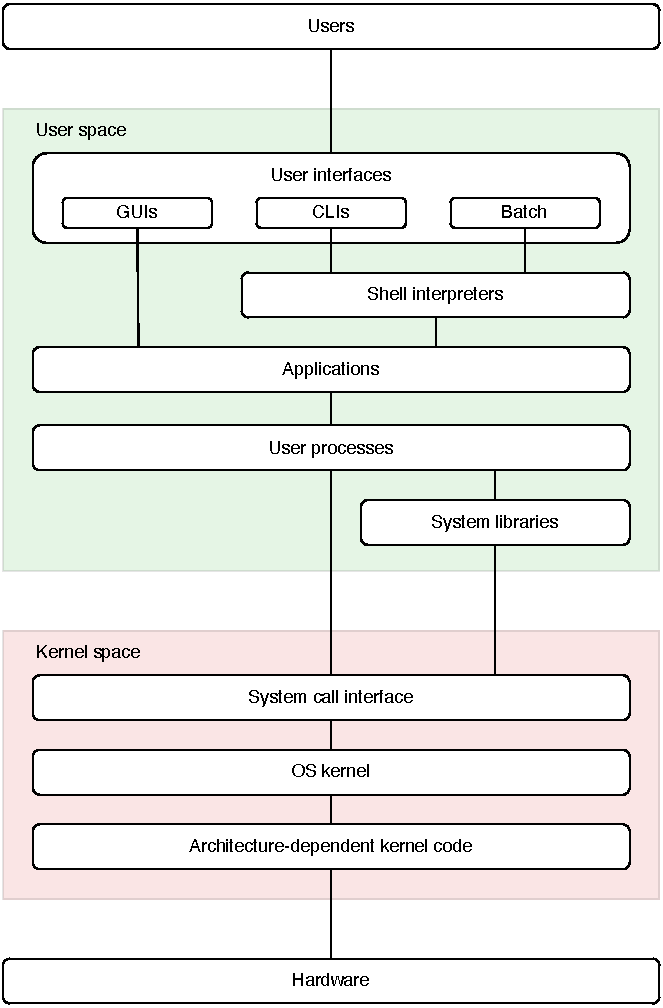
\includegraphics{assets/linux_os_structure.pdf}
    \caption{Linux OS architecture}
    \label{fig:linux_os_structure}
\end{figure}

Figure \ref{fig:linux_os_structure} provides a high-level overview of the Linux OS architecture.
Starting from the top of the diagram, users interact with the operating system though the user interface layer, which includes Graphical User Interfaces (GUIs), Command Line Interfaces (CLIs) and batch interfaces. GUIs provide elements for user visual interaction, such as windows, icons, buttons and menus. CLIs provide tools for text and command-based user interaction, allowing users to launch commands and scripts. Batch interfaces allow users to schedule commands to be executed at specific time or conditions.
User interfaces are the outermost user space layer and allow users to interact with both system and installed applications.
The term "user space" refers to the memory area where unprivileged user applications reside. 
Applications running in the user space are said to be running in "user mode", meaning they have limited access to system resources and are prevented from executing operations that could compromise the system's stability and security. \newline
Right below the user interface layer, shell interpreters connect CLIs and batch interfaces to the application layer by interpreting and executing commands.
The application layer includes both system and user-installed applications, running in user mode. Right below this layer, the process layer includes all active user processes, namely all instances of running applications. 
The process layer relies on system libraries as a simple, high-level programming interface to kernel functionalities. 
Below system libraries, the diagram depicts the kernel space, which is the memory area where the kernel and its modules reside. The kernel act as the core of the operating system, handling a wide range of critical tasks such as process scheduling, memory, file system and device management, I/O operation handling, network and inter-process communication management, system security enforcement, etc.
Software running in the kernel space runs in "kernel mode", meaning it has full access to system resources and can execute privileged operations.
The first kernel space layer is the system call interface, which serves as the abstraction layer between user and kernel space, providing a clean and secure way for user processes running in user mode to access kernel functionalities.
The OS kernel relies on architecture-dependent code to interact with the underlying hardware layer, which includes all the host physical components, such as the host CPU, memory, storage and network interfaces.

\section{Virtualization technologies}
Virtualization technologies are used to deploy applications in strictly isolated environments by running multiple virtual machines (VMs) on the same physical hardware.
Each VM consists in a full-fledged OS instance, with its own kernel and user space.
The software layer responsible for assigning physical resources to VMs is called hypervisor.
Depending on the hypervisor collocation, virtualization technologies can be divided into two main categories: bare metal (type 1) and type 2. 

\begin{figure}[htbp]
    \centering
    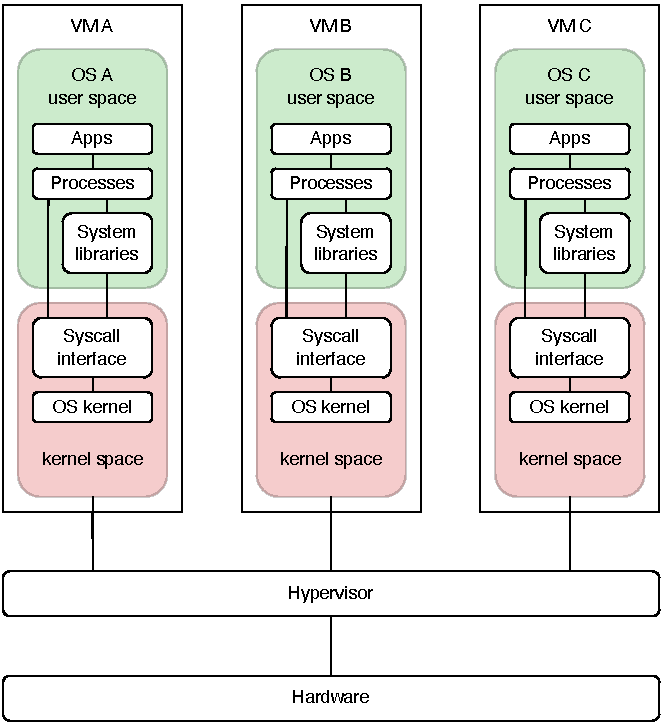
\includegraphics{assets/type_1_virtualization.pdf}
    \caption{Bare metal (type 1) virtualization environment}
    \label{fig:bare_metal_virtualization}
\end{figure}

\begin{figure}[htbp]
    \centering
    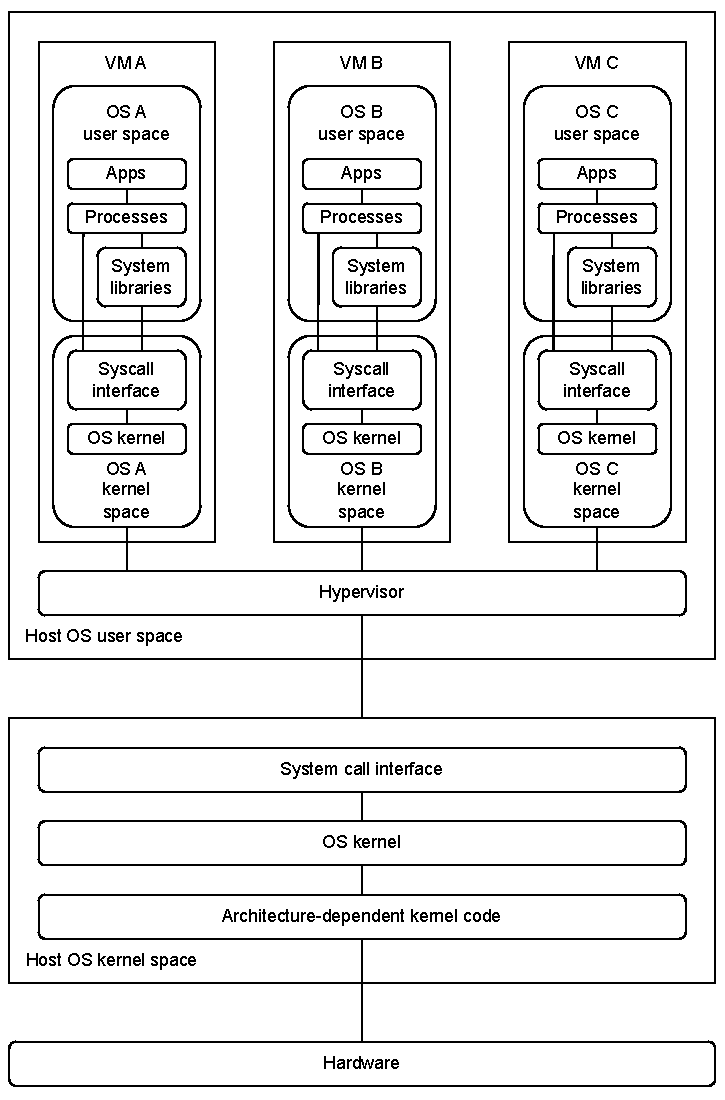
\includegraphics{assets/type_2_virtualization.pdf}
    \caption{Type 2 virtualization environment}
    \label{fig:tipe_2_virtualization}
\end{figure}

Figure \ref{fig:bare_metal_virtualization} shows a bare metal virtualization environment. 
The hypervisor runs directly on the hardware, implementing the virtualization layer by providing a virtualized representation of the physical hardware to each VM.
The diagram shows three VMs, each one running a different OS, having a different set of system libraries and running a different set of applications. 

Figure \ref{fig:tipe_2_virtualization} depicts a type 2 virtualization environment.
The hypervisor runs in the host OS user space, providing VMs with access to physical resources by redirecting system calls to the host OS system call interface. Three VMs are shown, each one running a different OS, having a different set of system libraries and running a different set of applications.
In a nutshell, the main difference between type 1 and type 2 virtualization resides in the hypervisor collocation: bare metal hypervisors run directly on the hardware, while type 2 hypervisors rely on the host OS kernel to access physical resources. 

Bare metal virtualization generally provides better performance and better VM isolation than type 2.
Nowadays, the most popular hypervisors are VMware ESXi, Microsoft Hyper-V and KVM (Kernel-based Virtual Machine).
All these technologies are widespread in cloud environments and are behind several famous cloud-based services like Amazon AWS, Microsoft Azure and Google Cloud Platform.

The diffusion of virtualization technologies allowed the adoption of complex cloud infrastructures following the IaaS or PaaS models \cite{stonemanLearnDockerMonth}.
According to the IaaS model, cloud providers offer only hardware and basic software resources while customers are responsible for the deployment, management and maintenance of applications.
The PaaS model, on the other hand, allows customers to use a complete production environment offered by cloud providers.
Neither models constitutes an optimal alternative in terms of costs and flexibility.
The IaaS model involves deploying each application component on a separate virtual machine. For this reason, each component must be managed and scaled manually, resulting in expensive and often underutilized VMs. However, this model provides excellent portability between different cloud platforms because the deployment is not cloud-service specific. On the other hand, according to the PaaS model, each component relies on specific cloud services offered by the providers. 
Although more flexible and less expensive than the IaaS model, PaaS deployments are much less portable as they exploit cloud platform-specific services.
 

\section{Linux containers}
Despite the term container gained popularity after the diffusion of Docker, the technology at its back has been in the engineering landscape since the introduction of Linux Containers (LXC) \cite{LinuxContainers} in 2008.
A Linux container is a group of Linux processes running in isolation that, unlike VMs, share the same host OS kernel. 
Despite simple from a theoretical perspective, isolating Linux processes in containers is not a trivial task since it requires reliable resource isolation techniques and a software layer capable of using them to group processes. 
The integration in the Linux kernel of \texttt{namespace} and \texttt{cgroups} isolation technologies in 2006 paved the way for the creation of such a layer, making LXC the first example of container runtime, namely a software capable of managing Linux containers by directly interfacing with the underlying host OS Linux kernel.
In other words, LXC provides a user space low-level API that, by using Linux kernel isolation features, allows grouping Linux processes in isolated sets.
LXC API is implemented as the \texttt{liblxc} C system library. 

Despite being powerful tools, container runtimes alone are not enough to obtain a full functioning containerized environment since they do not provide advanced tools to manage the entire container lifecycle.  
To this purpose, a higher-level software layer is needed, namely a container engine. 
By relying on the container runtime, container engines provide advanced tools for container creation, deletion, orchestration, networking, storage sharing, etc. 

\begin{figure}[htbp]
    \centering
    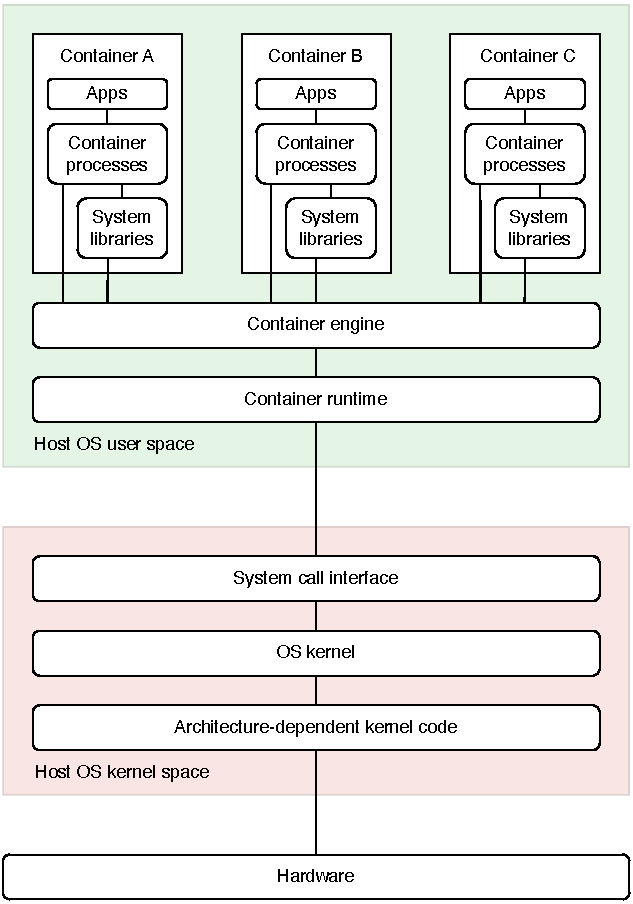
\includegraphics{assets/containerization.pdf}
    \caption{Containerized environment}
    \label{fig:containers}
\end{figure}

Figure \ref{fig:containers} illustrates a complete containerized environment.
Right above the container engine and runtime layers, the diagram shows three running containers, each one having a different set of system libraries and running a different set of processes in isolation. 
The container engine interfaces with the process layer while the container runtime handles the low-level interaction with the host OS kernel, using system calls to manage \texttt{namespaces} and \texttt{cgroups}. 
The host OS kernel space and the hardware layers are depicted as in figure \ref{fig:linux_os_structure}. 

\section{Comparison of Linux containers and virtual machines}
The introduction of Linux containers consisted in a radical departure from traditional virtualization-based deployments, namely IaaS and PaaS: the application to be deployed is no longer deployed as a monolithic entity on a single VM, but as a set of orchestrated components, each one running in a separate container. 
Container-based deployment addresses the main problems of traditional IaaS and PaaS models, combining PaaS flexibility with IaaS portability.

Despite these clear advantages, containers do not play the role of "silver bullets" in the field of software production. 
Containers are usually ephemeral, lightweight and portable wrappers around Linux processes \cite{kaneDockerRunningShipping2023}, 
no more. Virtual machines are an abstraction of physical hardware. 
This difference in philosophy reflects on the use cases of the two technologies. \newline
Virtual machines are often long-lived, with a minimum lifespan of days or weeks. 
For this reason, virtualization is still the solution of choice when a deployment is expected to be long-lived and, in a sense, "stable".
Moreover, virtualization is used when a small set of cloud applications require different operating systems (or different OS versions) \cite{bernstein2014containers}. 
The number of VMs running on a host is usually limited to a few units since each VM consists in a full-fledged OS instance.
Containers are significantly smaller in size: an host can run hundreds or even thousands of containers, each one representing a single application component.
By having lower overhead, higher performance and faster startup and stop times than virtual machines \cite{felter2015updated,chae2019performance}, containers are the perfect solution when the set of services to be deployed is vast but far more homogeneous.
Despite being isolated from each other, the isolation degree of containers is significantly lower than that of virtual machines. While limits can be enforced on the resources containers can access, they usually share CPU and memory on the host system, as co-located UNIX processes do. 

\section{Docker}
The introduction of LXC in 2008 was a fundamental step forward the adoption of containerization technologies. However, LXC is only a container runtime, it does not provide advanced tools for managing the entire container lifecycle. \newline
At the time of its first release, on March 20, 2013,
Docker
provided a container engine that, by using LXC as a container runtime, offered a higher-level API for container management.
On March 13, 2014, with the release of Docker version 0.9, LXC was replaced with a new container runtime, \texttt{libcontainer}, still exploiting Linux kernel isolation features but entirely written in Go.
Nowadays, Docker is way more than a container engine: it's a complete containerization framework that provides a container engine, a container runtime and a set of tools for container sharing and orchestration.
By initially extending LXC and then transitioning to \texttt{libcontainer}, Docker brought Linux containers to the masses, becoming the de-facto standard for containerization. 

\section{Docker images}
Docker images play a key role in the Docker ecosystem by promoting container distribution and sharing.
They are the templates from which Docker containers are created \cite{WhatIsDocker}. 
In other words, an image is a container snapshot. It's an object that contains an OS filesystem, an application component and all the dependencies it needs to be deployed in isolation. 
From a deployment perspective, images are similar to VM templates, from a development perspective, images are similar to Object Oriented Programming classes from which objects (Docker containers) are instantiated.

\section{Docker architecture}

\begin{figure}[htbp]
    \centering
    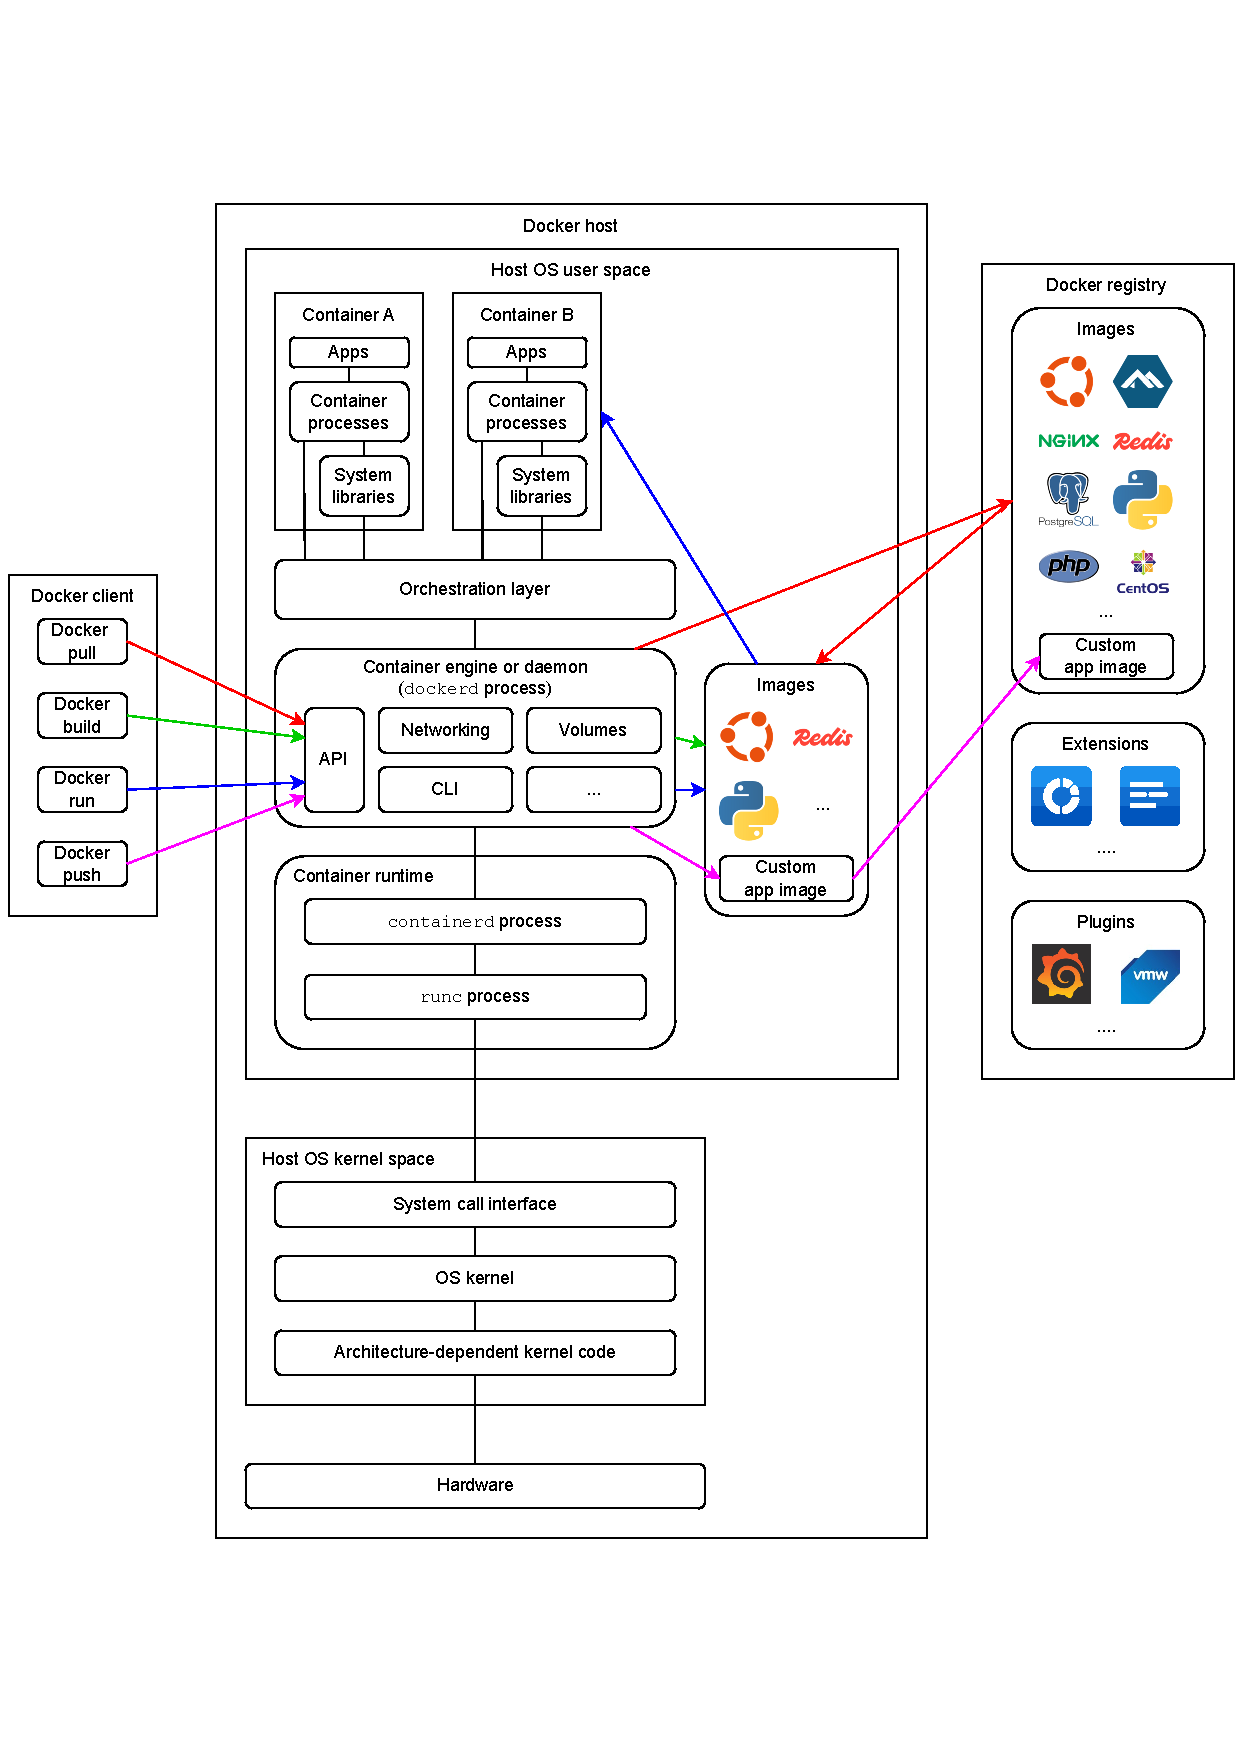
\includegraphics[width=1\textwidth]{assets/docker.pdf}
    \caption{Docker architecture}
    \label{fig:docker_architecture}
\end{figure}

Docker fundamental structure consists of a client-server architecture. 
As figure \ref{fig:containers} shows, the Docker client talks to the container engine through a REST API. The container engine is responsible of building, running and distributing Docker containers. For this reason, is also called Docker daemon.
A Docker client can be a CLI or a GUI running on the same machine as the daemon or on a remote one.
The Docker client-daemon REST API, leverages UNIX sockets or a network interfaces, depending whether the client and daemon are running on the same machine or not.

The Docker daemon consists of the \texttt{dockerd} process that, by running in the Docker host user space, listens for Docker API requests from the clients and manages Docker images, containers, networks and volumes accordingly. 

The Docker client consists of the \texttt{docker} command, followed by a subcommand specifying the action to be performed on Docker entities, such as building an image (\texttt{docker build}), running a container (\texttt{docker run}), stopping a container (\texttt{docker stop}), etc. 
These commands are forwarded to the Docker daemon through the REST API and are partially shown in figure \ref{fig:docker_architecture}.

A standard Docker installation provides also basic orchestration tools, such as \texttt{docker-compose} and \texttt{docker swarm}, depicted as the orchestration layer in figure \ref{fig:docker_architecture}.

The Docker registry stores Docker images to promote their sharing and distribution. A registry can be private (widespread in enterprise contexts) or public. The most famous public registry is Docker Hub, an online repository backed by Docker Inc. and sustained by an extensive community of developers. 
The addition of registries can be considered as the major extension offered by Docker to the LXC technology. Figure \ref{fig:docker_architecture} depicts a Docker registry as a separate, maybe "remote" entity containing Docker images (such as Ubuntu, Redis, Alpine Linux, etc). However, a registry can be co-located with the Docker daemon as well.

The Docker container runtime operates at the lowest level, still in the user space. As explained, it interfaces with the host OS kernel to start and stop containers by managing all OS constructs such as \texttt{namespaces} and \texttt{cgroups}.
The runtime is implemented in a tiered fashion. The low-level runtime, \texttt{runc}, is the reference implementation of the OCI runtime specification. Its duty is to interface with the underlying Linux host kernel to start and stop containers. The high level runtime, \texttt{containerd}, manages the entire container lifecycle, including pulling images from registries and managing \texttt{runc} instances. \newline
A typical Docker installation has a single \texttt{containerd} process instructing \texttt{runc} to start and stop containers. \texttt{runc} processes are typically short-lived, terminating as soon as a container is started or stopped. \newline
\texttt{dockerd} is located above \texttt{containerd} and performs higher-level tasks such as exposing the Docker REST API, managing images, networks and volumes. 

\section{Benefits of Docker}
The main benefits of Docker:
\begin{itemize}
    \item \textbf{Reproducibility and portability}: Docker containers are immutable and can be easily shared as artifacts between different environments, ensuring that the containerized application will run consistently on any machine. The application is usually deployed as a single container image, which contains all the dependencies and files it needs to run. 
    \item \textbf{Isolation}: containers are - or should be - isolated from each other and from the host system, reducing the risk of dependency conflicts between applications and granting a good level of security.
    \item \textbf{Resource efficiency by preserving hardware-software abstraction}: containers share the same host OS kernel. For this reason, containerization exhibit a lower overhead with respect to virtualization. Hardware-software abstraction, usually desired in enterprise solutions, is preserved (to a minor extent compared to virtualization technologies).
    \item \textbf{Scalability}: Docker makes it easier to scale applications, especially if they are deployed by orchestrating microservices. Each service is usually deployed as a group of containers, that can be easily scaled up or down according to the load. 
    \item \textbf{Low configuration overhead}: Docker simplifies the process of setting up development and production environments, simplifying an error-prone and time-consuming process.
\end{itemize}












